\newpage

\section{TLS/SSL VPN Configuration}

This section details the configuration of the TLS-based VPN connection using OpenVPN as the client software. The TLS implementation provides session-layer security with certificate-based authentication and encryption, establishing a secure tunnel between the client container and the SoftEther VPN server.

\subsection{OpenVPN Client Setup}

OpenVPN is a robust and highly configurable VPN solution that uses SSL/TLS for key exchange and encryption. It operates in user space and provides flexibility in configuration and deployment.

\subsubsection{Software Installation}

The OpenVPN client software was installed during the initial container configuration. To verify the installation:

\begin{lstlisting}[language=bash]
# Verify OpenVPN installation
openvpn --version

# Check OpenVPN capabilities
openvpn --show-ciphers | head -10
openvpn --show-digests | head -10

\end{lstlisting}

\subsubsection{Certificate and Key Management}

Unlike IPSec's pre-shared key approach, OpenVPN uses X.509 certificates for authentication, providing stronger security and better scalability.

\noindent
\\
\textbf{Required Certificate Files:}

\begin{itemize}
    \item \textbf{CA Certificate:} Root certificate to verify server authenticity
    \item \textbf{Client Certificate:} Client's public key certificate (not used in this setup)
    \item \textbf{Server Verification:} Server certificate validation parameters
    \item \textbf{User Credentials:} Username and password for authentication
\end{itemize}

\subsection{Certificate and Credential Management}

The TLS-based VPN uses a combination of certificate-based server authentication and username/password client authentication.

\subsubsection{User Credentials}

The client authenticates using username and password stored in a credentials file:

\begin{lstlisting}[language=bash]
# /client/credentials.txt
user1
ciao
\end{lstlisting}

\noindent
\textbf{Authentication Details:}
\begin{itemize}
    \item \textbf{Username:} user1 (matches SoftEther server user configuration)
    \item \textbf{Password:} ciao (matches server's user password)
    \item \textbf{Security:} File should have restricted permissions (600) in production
    \item \textbf{Authentication Layer:} These credentials are used for application-layer authentication after TLS handshake completion, not during the handshake itself
\end{itemize}

\subsection{OpenVPN Configuration Analysis}

The OpenVPN configuration file (*.ovpn) contains all parameters necessary for establishing the TLS VPN connection.

\subsubsection{Complete Configuration File}

\begin{lstlisting}[language=bash]
# /client/softether.ovpn
client                                   # Client mode
dev tun                                  # TUN interface
proto tcp                                # TCP transport protocol
remote 203.0.113.1 443                   # Server IP and port
resolv-retry infinite                    # Retry DNS resolution
nobind                                   # Don't bind local port
persist-key                              # Keep keys in memory
persist-tun                              # Keep TUN interface
ca ca.crt                                # CA certificate file
remote-cert-tls server                   # Verify server cert
verify-x509-name da3af5075c51 name       # Verify server CN
auth-user-pass credentials.txt           # Username/password file
cipher AES-128-CBC                       # Encryption cipher
data-ciphers AES-128-CBC                 # Allowed ciphers
mssfix 1450                              # MSS clamping for MTU
verb 4                                   # Verbosity level
\end{lstlisting}

\noindent
\textbf{Configuration Parameter Analysis:}

\begin{itemize}
    \item \textbf{Connection Type:} Client mode with TCP transport for reliability
    \item \textbf{Interface:} TUN device for Layer-3 IP tunneling
    \item \textbf{Server Details:} Connects to SoftEther server on port 443 (HTTPS)
    \item \textbf{Authentication:} Dual authentication with certificates and credentials
    \item \textbf{Encryption:} AES-128-CBC cipher for data encryption
    \item \textbf{Network Optimization:} MSS fixing to prevent fragmentation issues
\end{itemize}

\subsubsection{Security Features}

The OpenVPN configuration implements several security mechanisms:

\begin{enumerate}
    \item \textbf{Server Authentication:} X.509 certificate ensures server identity during TLS handshake
    \item \textbf{Certificate Name Verification:} CN prevents man-in-the-middle attacks during TLS handshake
    \item \textbf{Strong Encryption:} AES-128-CBC provides confidentiality
    \item \textbf{Transport Security:} TLS transport layer provides additional protection
\end{enumerate}

\noindent
\textbf{Authentication Process Clarification:} The TLS handshake process only involves server certificate validation. The user credentials (user1/ciao) are transmitted and validated within the established TLS tunnel as an additional application-layer authentication step, providing defense-in-depth security.

\subsection{TLS Handshake and Connection}

The TLS VPN establishment process involves multiple phases, including TLS handshake, authentication, and tunnel creation.

\subsubsection{Connection Establishment Process}

To establish the TLS VPN connection:

\begin{lstlisting}[language=bash]
# Navigate to client configuration directory
cd /client

# Start OpenVPN connection
openvpn --config softether.ovpn

# Alternative: Run in background
openvpn --config softether.ovpn --daemon
\end{lstlisting}

\subsubsection{Connection Verification}

Successful TLS tunnel establishment can be verified through several indicators:

\begin{lstlisting}[language=bash]
# Check TUN interface creation
ip addr show | grep tun

# Test connectivity to SoftEther SecureNAT
ping 192.168.30.1

# Check assigned VPN IP address
ip addr show tun0
\end{lstlisting}

\noindent
\textbf{Successful Connection Indicators:}
\begin{itemize}
    \item "Initialization Sequence Completed" message appears
    \item TUN interface (tun0) is created with VPN IP address
    \item Routes are added for VPN traffic
\end{itemize}

\subsection{Encrypted Traffic Analysis}

TLS-based VPNs provide comprehensive encryption at the session layer, protecting all tunneled traffic.

\subsubsection{Wireshark Packet Analysis}

To observe TLS/OpenVPN traffic in detail, it is highly recommended to open a Wireshark instance on one of the network cables connecting the client and server infrastructure. This allows real-time analysis of the VPN establishment and data transmission phases.

\begin{figure}[H]
\centering
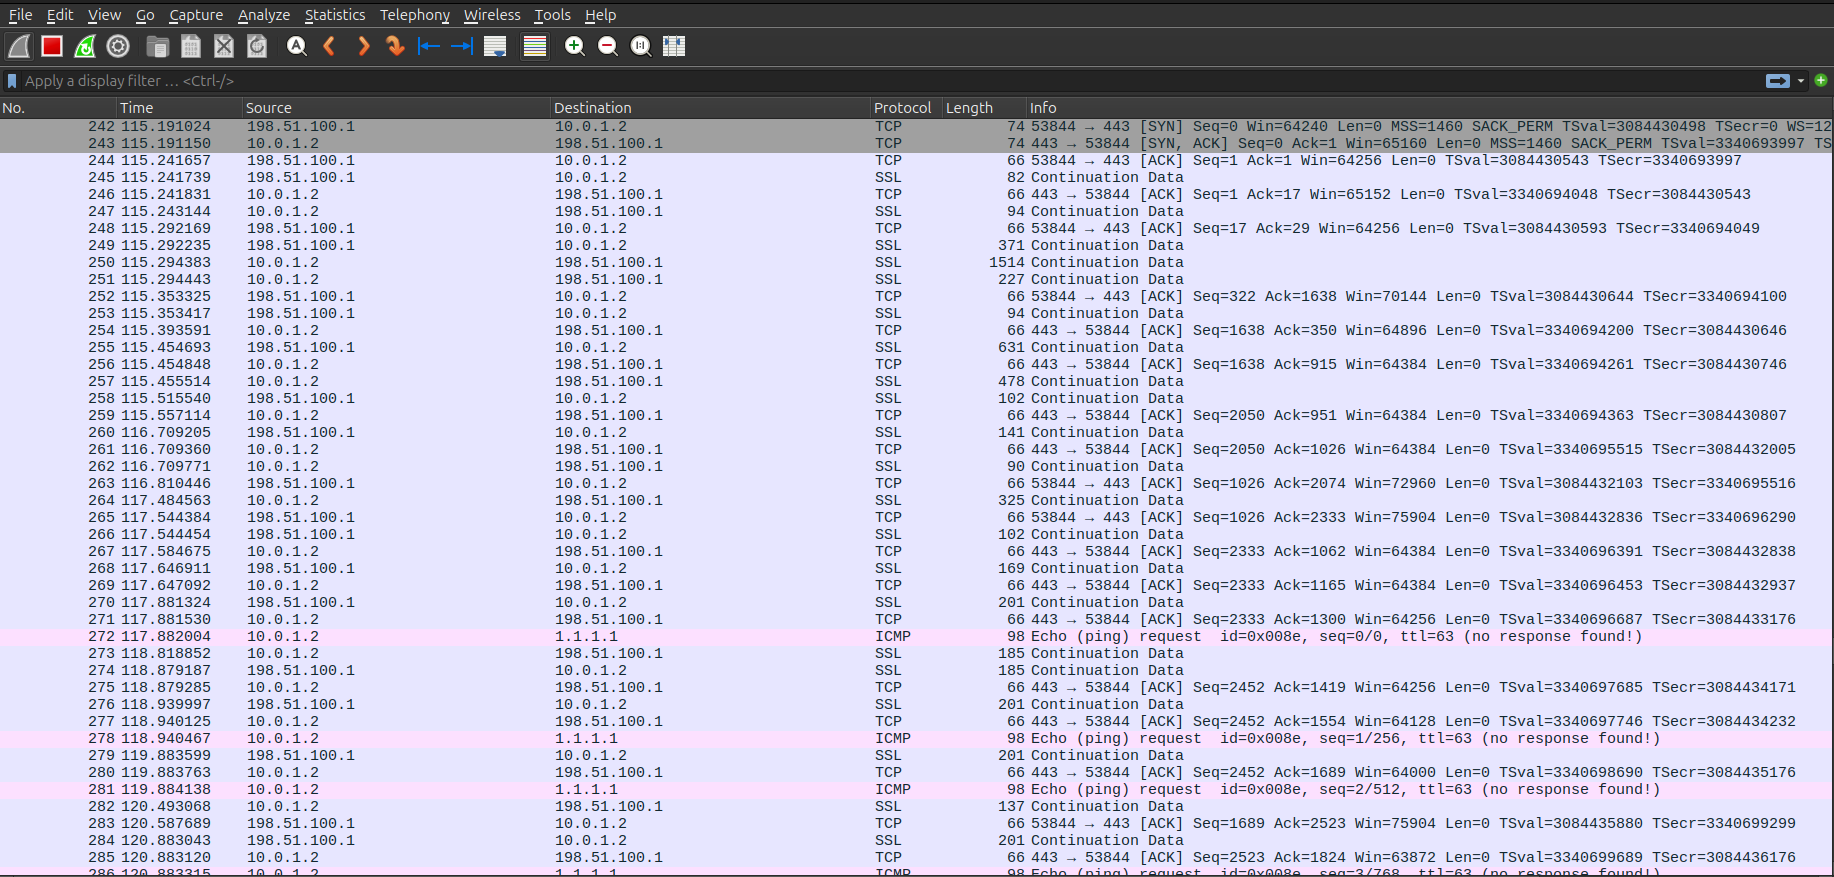
\includegraphics[width=\textwidth]{../resources/Images/TLS_Packets.png}
\caption{TSL VPN Packets in Wireshark}
\label{fig:tls_packets}
\end{figure}

\noindent
\\
\textbf{TLS Handshake and Connection Establishment Phase:}

\noindent
During the initial TLS VPN connection setup, Wireshark will capture SSL/TLS handshake packets and OpenVPN protocol messages. You can start the Wireshark capture instance by right clicking on a wire in GNS3, and then selecting "Start Capture". In this phase you will observe:

\begin{itemize}
    \item \textbf{TCP Connection:} Initial TCP connection establishment on port 443
    \item \textbf{TLS Handshake packets:} SSL/TLS negotiation between client and server
    \item \textbf{Certificate Exchange:} Server certificate transmission and validation
\end{itemize}

\noindent
\\
\textbf{Active Tunnel Communication Phase:}

\noindent
Once the TLS VPN tunnel is established and active communication begins, the packet capture will show encrypted SSL data packets. 

\noindent
\\
\textbf{Important Traffic Flow Observation:}

\noindent
When the client initiates communication (such as a ping command) to destinations beyond the VPN server, the ping message travels through the entire TLS tunnel to be decapsulated and transmitted by the server on behalf of the client. This means that when observing traffic with Wireshark, the source address of the ping message that appears in the packet capture will not be the original client address, but rather the SoftEther server's SecureNAT IP address.

\noindent
This behavior occurs because:
\begin{itemize}
    \item The client's traffic is completely encapsulated within the TLS tunnel
    \item The SoftEther server decapsulates the traffic and forwards it using its own SecureNAT functionality
    \item The server acts as a NAT gateway, replacing the source IP address with its own
    \item External destinations see traffic originating from the VPN server, not the original client
\end{itemize}

\begin{lstlisting}[language=bash]
# Test communication to generate OpenVPN traffic and observe source translation
ping 192.168.30.1  # From client to SoftEther SecureNAT
\end{lstlisting}


\subsubsection{Connection Termination}

To properly terminate the VPN connection:

\begin{lstlisting}[language=bash]
# Find OpenVPN process
ps aux | grep openvpn

# Gracefully terminate connection
kill -SIGTERM <openvpn_pid>

# Force termination if necessary
kill -SIGKILL <openvpn_pid>

# Verify interface cleanup
ip addr show | grep tun
\end{lstlisting}

\noindent
The TLS-based VPN configuration is now complete and ready for testing. This implementation provides a user-space alternative to the kernel-based IPSec solution, demonstrating different approaches to achieving secure network connectivity. The next section will verify both VPN implementations and analyze their traffic characteristics.
